%% V1.0
%% by Gabriel Garcia, gabrcg@gmail.com
%% This is a template for Udacity projects using IEEEtran.cls

%% Be Udacious!

\documentclass[10pt,journal,compsoc]{IEEEtran}

\usepackage[pdftex]{graphicx}
\usepackage{cite}
\hyphenation{op-tical net-works semi-conduc-tor}


\begin{document}

\title{Where Am I}

\author{Seyfi Gozubuyuk}

\markboth{Localization project, Robotics Nanodegree Program, Udacity}%
{}
\IEEEtitleabstractindextext{%

\begin{abstract}
In this project, the aim is to utilize ROS packages to accurately localize a mobile robot inside a provided map inside a provided map in the Gazebo and RViz simulation environments. The overview of the tasks can are as follows, building two mobile robots for simulated tasks, creating a ROS package that utilizes AMCL package, exploring specific parameters.
\end{abstract}

% Note that keywords are not normally used for peerreview papers.
\begin{IEEEkeywords}
Robot, IEEEtran, Udacity, \LaTeX, Localization, ROS, AMCL, Robot Model.
\end{IEEEkeywords}}


\maketitle
\IEEEdisplaynontitleabstractindextext
\IEEEpeerreviewmaketitle
\section{Introduction}
\label{sec:introduction}

\IEEEPARstart{T}{he} problem is to localize the robot in a known map environment. It is critical to know the exact location of the robot, to create a path from the starting point to the goal. It is also crucial to localize the robot to prevent any collision with obstacles.\\
Noise from the sensors and the actuators makes it harder to estimate the robot position. There is a need for the location algorithms, to decrease the uncertainty caused by the noise. The most common algorithms are Kalman Filter and Monte Carlo Localization (Particle Filter). This project test the Adaptive Monte Carlo Localization with two different robot models. The Udacity Bot and the xbot. The project includes building the robot models and tuning the parameters. The environment contains Gazebo and RViz on ROS Kinetic. The ROS packages required to run this project are AMCL, move base, map server and navigation.


\section{Background}
The problem is to localize the robot, as mentioned earlier. The map is known; however, the sensors are not precise. There is noise to affect the measurements coming from the sensors, and the controls are not perfect to move the vehicle to the desired location. Therefore, we need to apply some techniques to use noise measurements.

\subsection{Kalman Filters}
Kalman Filters use noisy measurements and the actuation commands to estimate the location of the robot. There are two steps in Kalman Filters. They are predict and update. Predict step forecast the position after actuation command is applied, whereas the update step uses the measurements to update the location.
Kalman filters need to have Gaussian distributions to work. Therefore only linear operations are allowed on the probability. \\
Since the robot model is not entirely linear, there is a need for transforming nonlinear equations to linear equations. Taylor Series is the method for linear approximation. With linearization, the Kalman Filter become Extended Kalman Filter. \cite{wiki:kf}

\subsection{Particle Filters}
Particle Filter, also known as Monte Carlo Localization, starts with randomly generating particles. Each particle represents a possible location for the robot. The steps are similar to the Kalman Filter. After the motion, the position of each particle updates, and the uncertainty increases. After the measurements come from the sensors, the algorithm performs another update and the uncertainty decreases.\cite{wiki:pf}
\subsection{Comparison / Contrast}
Particle Filter can work with any distribution whereas Kalman Filter only works with a Gaussian distribution. Particle Filter takes raw measurements; however, Kalman Filter requires landmarks. The posterior is particles for Particle Filter and Gaussian for Kalman Filter. Kalman Filter is more efficient and provides more resolution; on the other hand Particle Filter is easier to implement and more robust. Only Particle Filter has Memory and Resolution control and can provide a solution for Glocal Localization. Particle Filter has Multimodal Discrete state space, and Kalman Filter has unimodal continuous.

\section{Simulations}
The simulation environment consists of ROS (Kinetic), Gazebo and RViz. The ROS packages are AMCL, move base, map server, and navigation. There are two different robot models to test on the simulation.

\subsection{The Udacity Bot}
The Udacity Bot has the robot model that described in the lesson. The robot has a chassis, two casters, two wheels, a laser sensor and a camera. Figure~\ref{fig:ubotgaz} and Figure~\ref{fig:ubotrvz} shows the Udacity bot in Gazebo and RViz.

\begin{figure}[thpb]
      \centering
      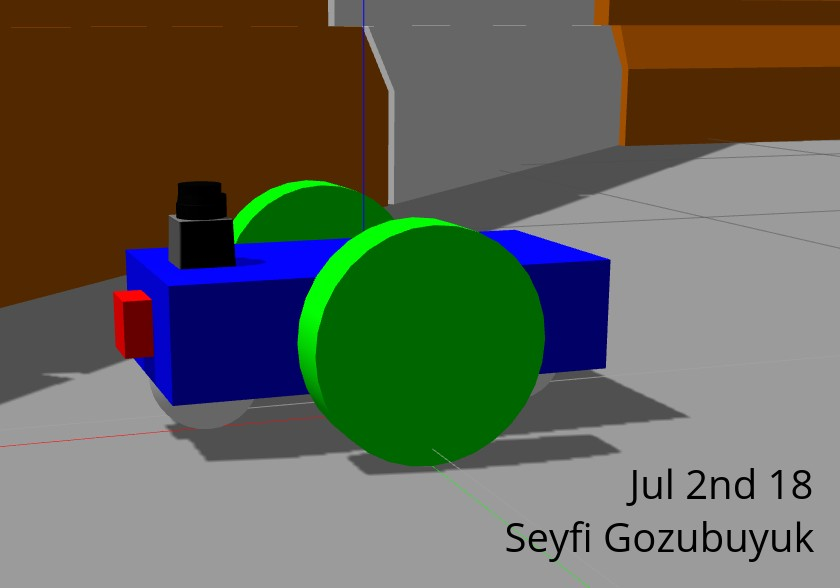
\includegraphics[width=\linewidth]{figures/UdacityBotGazebo.png}
      \caption{Udacity Bot in Gazebo}
      \label{fig:ubotgaz}
\end{figure}

\begin{figure}[thpb]
      \centering
      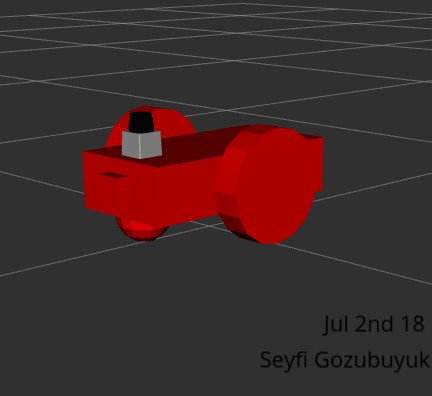
\includegraphics[width=\linewidth]{figures/UdacityBotRViz.png}
      \caption{Udacity Bot in RViz}
      \label{fig:ubotrvz}
\end{figure}

\subsection{The xbot}
The xbot is the slightly modified version of the Udacity Bot. It has a sensor base link which is in a rectangular box shape. This link is connected to the chassis and the laser sensor and the camera. Figure~\ref{fig:xbotgaz} and Figure~\ref{fig:xbotrvz} shows the xbot in Gazebo and RViz.

\begin{figure}[thpb]
      \centering
      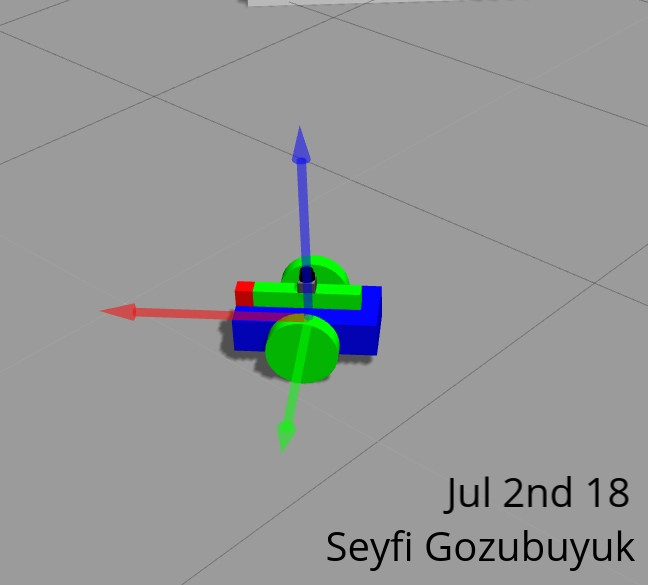
\includegraphics[width=\linewidth]{figures/xbotGazebo.png}
      \caption{xbot in Gazebo}
      \label{fig:xbotgaz}
\end{figure}

\begin{figure}[thpb]
      \centering
      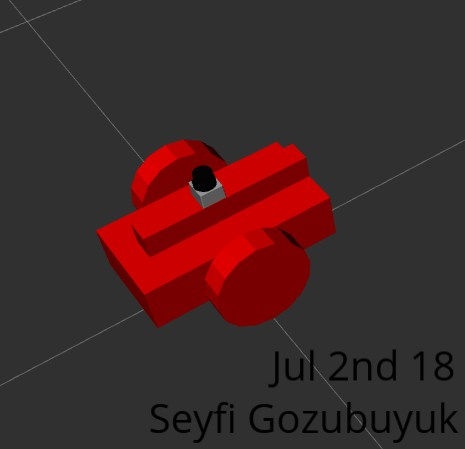
\includegraphics[width=\linewidth]{figures/xbotRViz.png}
      \caption{xbot in RViz}
      \label{fig:xbotrvz}
\end{figure}


\subsection{Achievements}
The Udacity bot and the xbot were able to reach the goal location. However, Udacity first went in the opposite direction to find a way to goal. After recognizing there was no way to goal, they turned back and the reach to the target. xbot directly moved in the correct direction; however, it moves in a curvy path.

% Robot Models
\subsection{Benchmark Model}
\subsubsection{Model design}
The main part of the Udacity bot is the chassis. It has a box shape with dimensions 0.4 x 0.2 x 0.1. It has two casters, one at -0.15 0 -0.05 and the other at 0.15 0 -0.05. There are two wheels connected to the chassis at 0 -0.15 0 and 0 +0.15 0. //
The laser sensor located at position relative to the chassis 0.15 0 0.085. It has a cubic shape with length 0.1. The camera sensor is connected to the chassis at 0.2 0 0, and it has a cubic shape with lenght 0.05.
The difference between the xbot and the Udacity bot is the link named sensor\textunderscore base. The camera and the laser sensors are connected to this link. The link has the dimensions of 0.3 0.05 0.05. It is connected to the chassis at location 0 0 0.075. The camera is connected to sensor\textunderscore base at 0.175 0 0 and the laser sensor connected to the sensor\textunderscore base at 0 0 0.05.

\subsubsection{Packages Used}
The packages used are as follows:
\begin{itemize}
\item ros-kinetic-navigation
\item ros-kinetic-map-server
\item ros-kinetic-move-base
\item ros-kinetic-amcl
\end{itemize}

Figure~\ref{fig:ubotgrp} and Figure~\ref{fig:xbotgrp} shows the topics for the Udacity Bot and the xbot.


\begin{figure}[thpb]
      \centering
      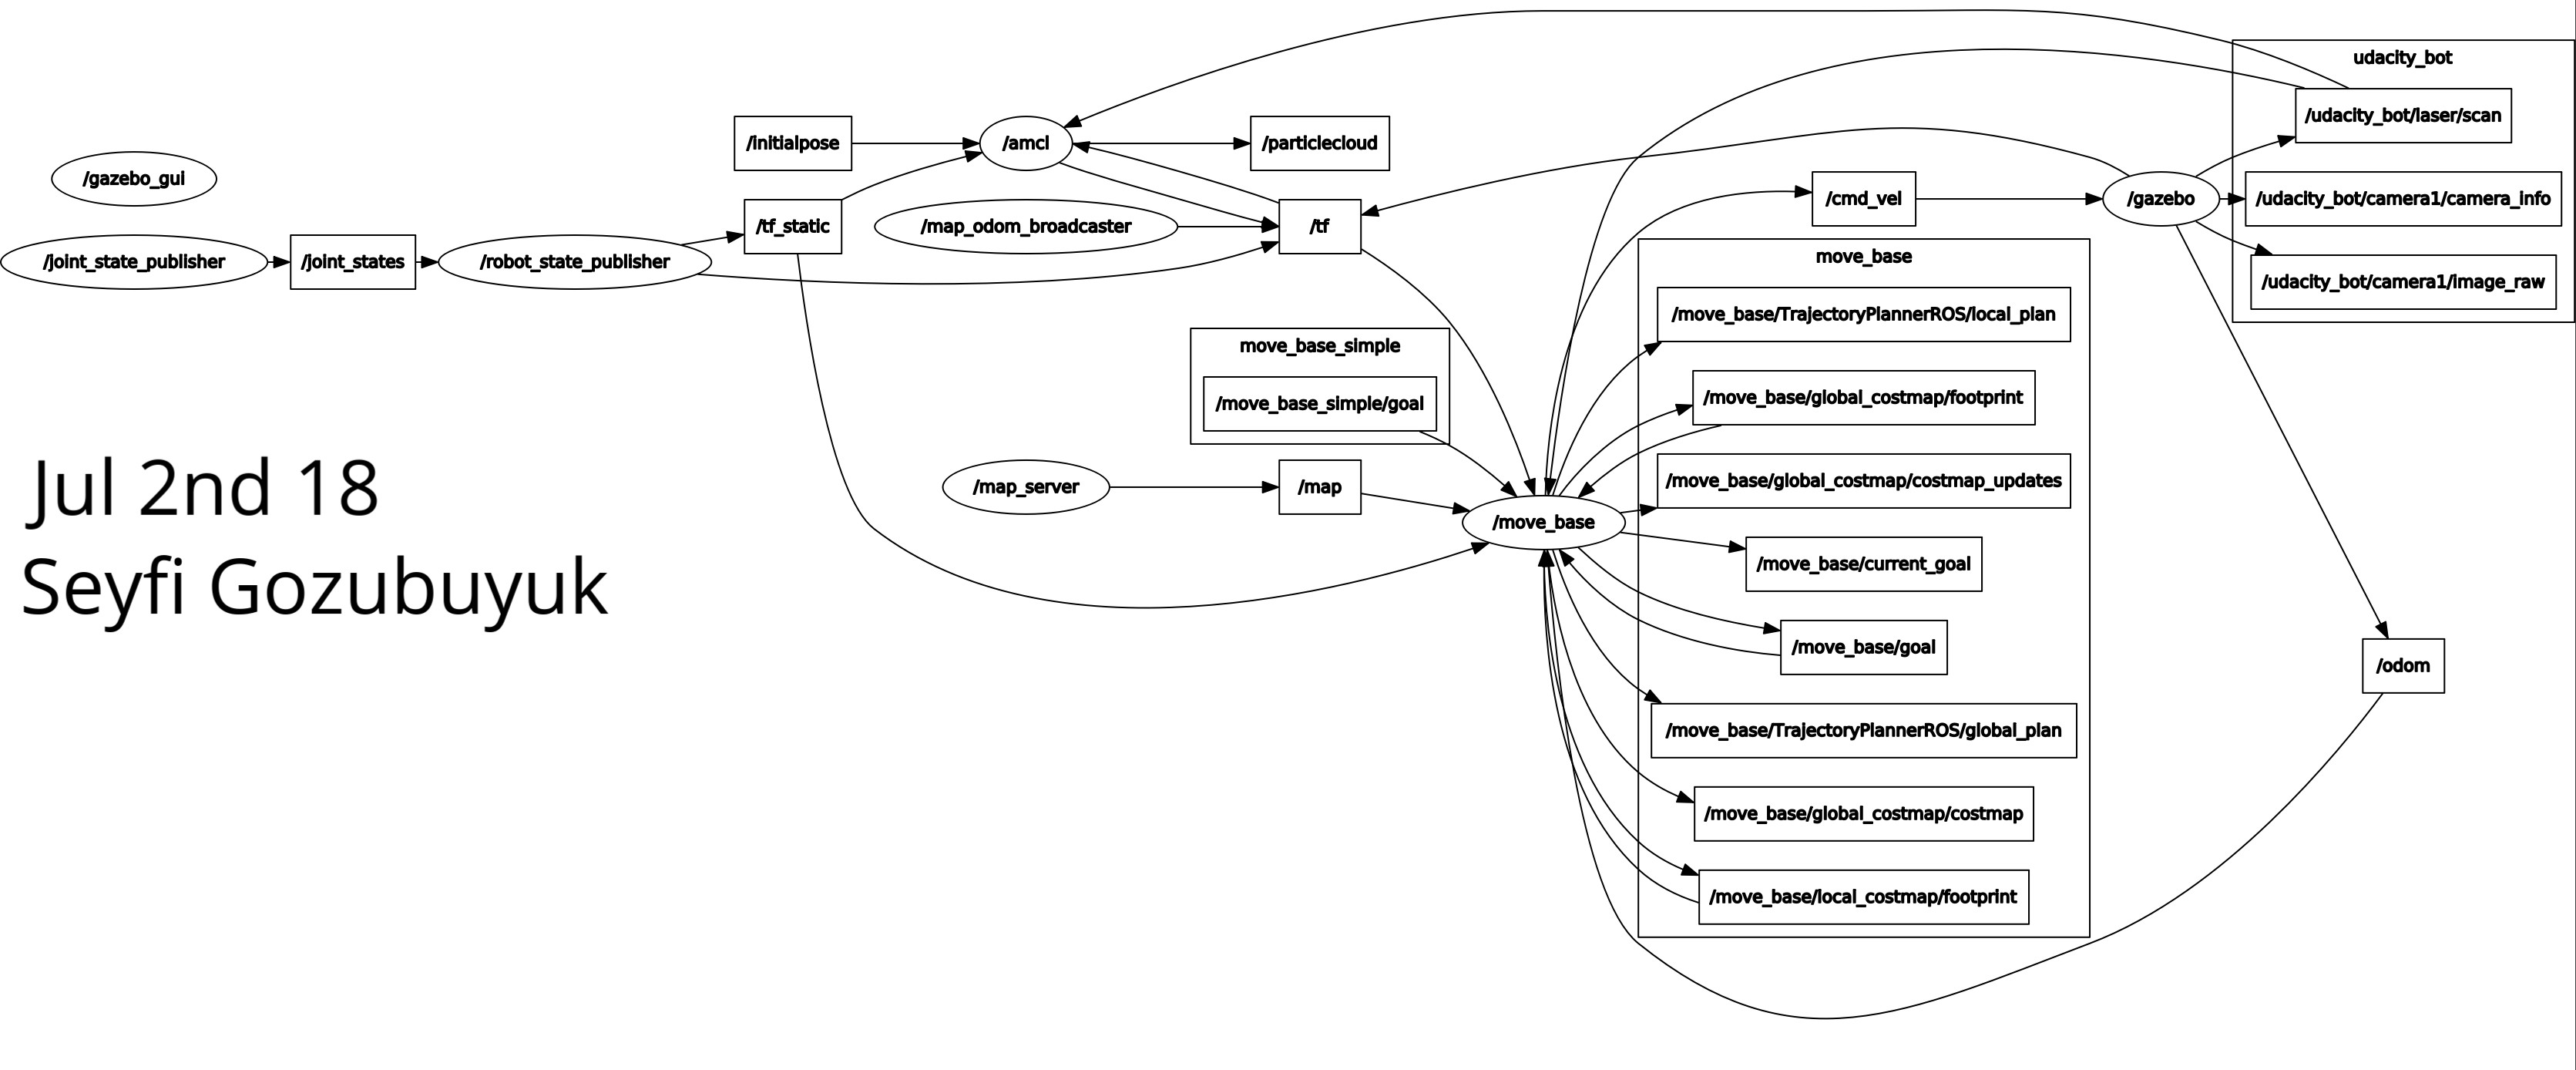
\includegraphics[width=\linewidth]{figures/rosgraph_ubot.png}
      \caption{Udacity Bot Rosgraph}
      \label{fig:ubotgrp}
\end{figure}

\begin{figure}[thpb]
      \centering
      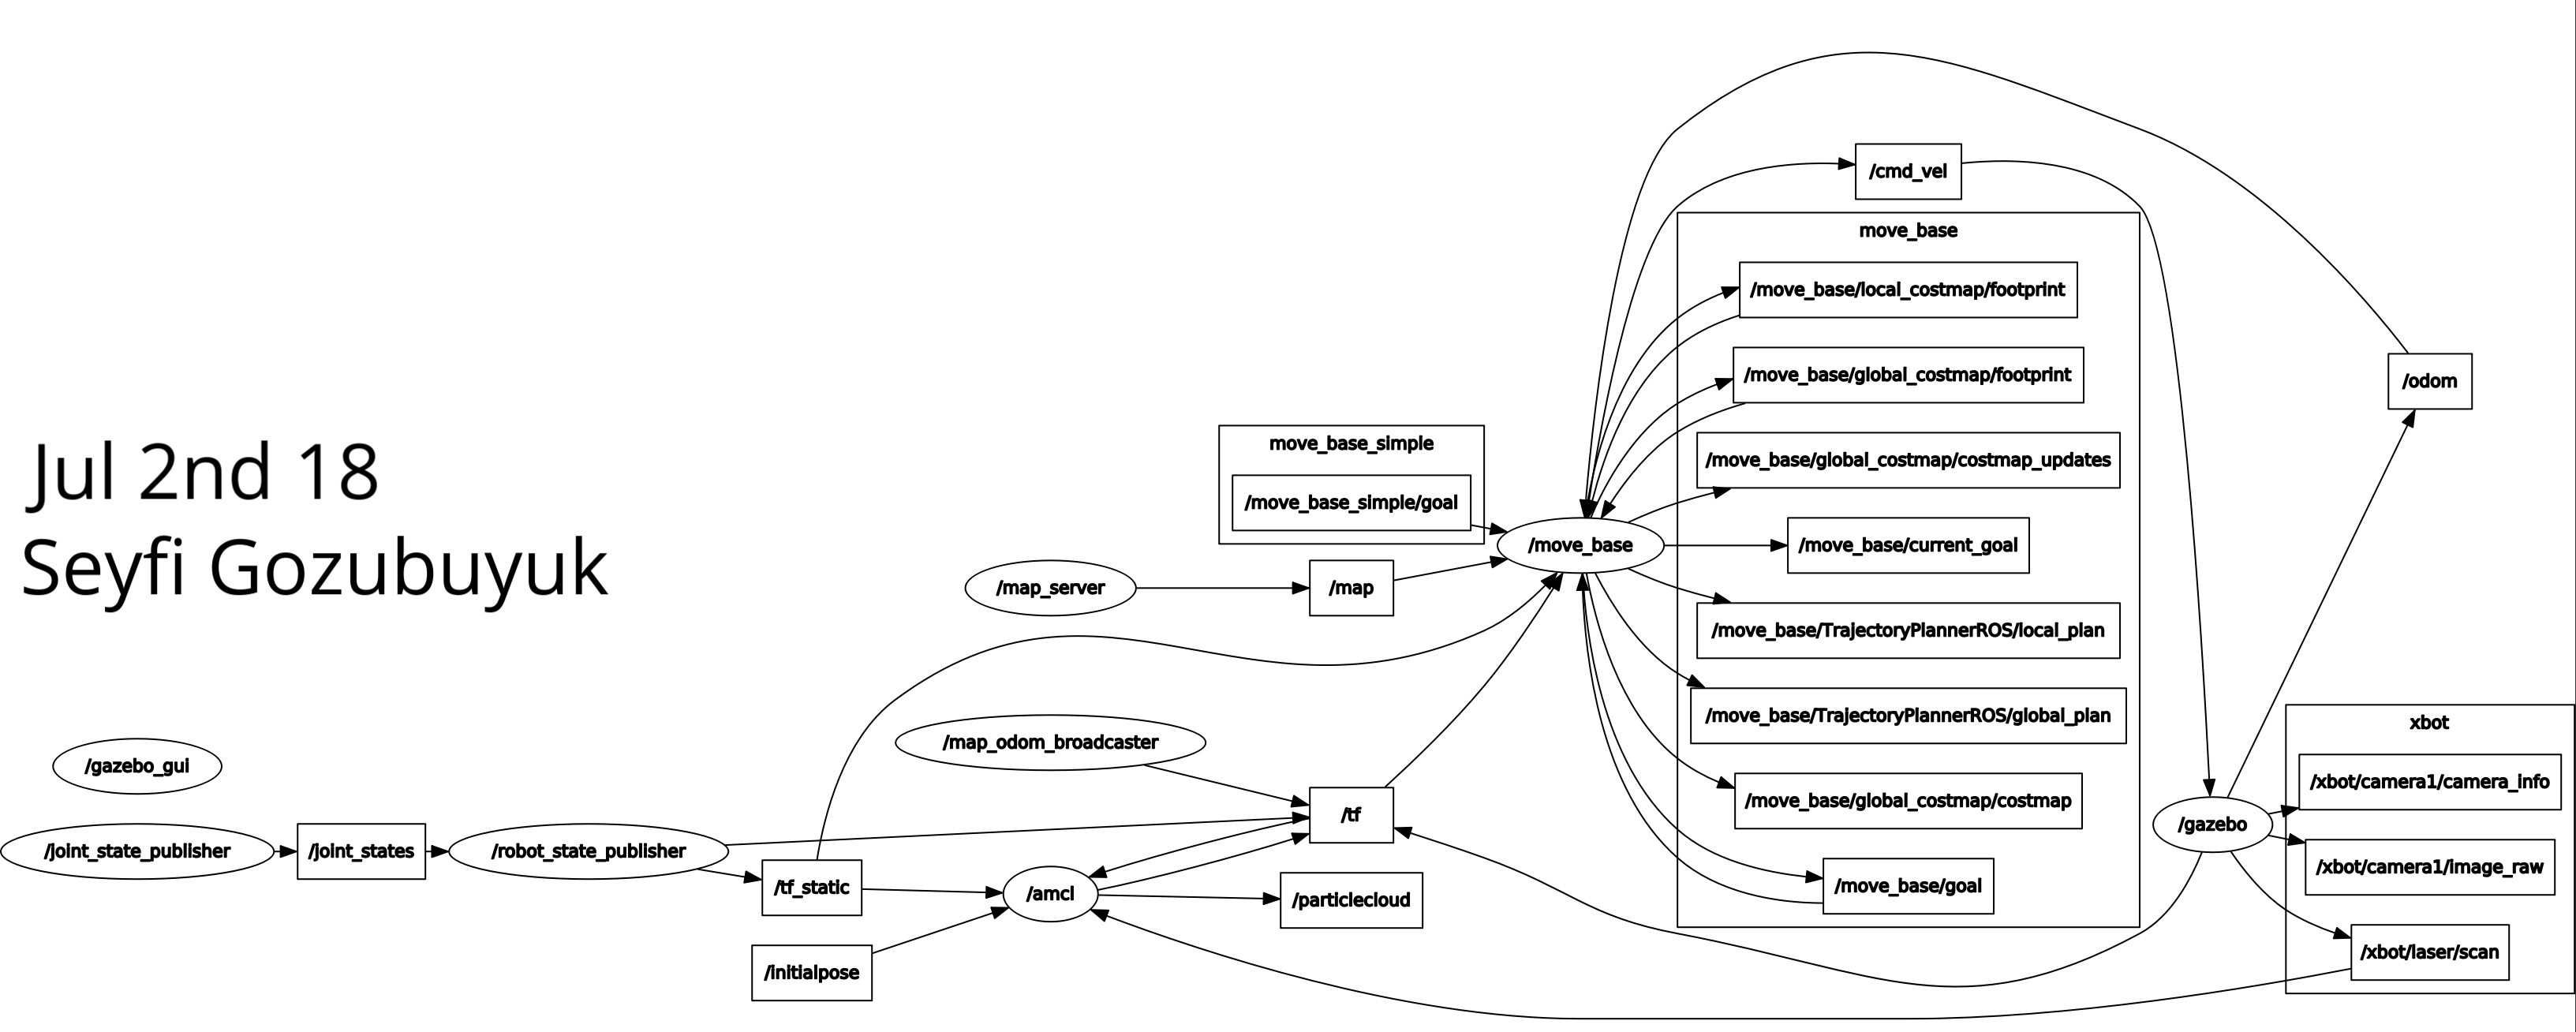
\includegraphics[width=\linewidth]{figures/rosgraph_xbot.png}
      \caption{xbot Rosgraph}
      \label{fig:xbotgrp}
\end{figure}

\subsubsection{Parameters}
The AMCL node parameters for Udacity bot is given in Table~\ref{table:amcl_params_ubot}\cite{rosnavgui}.
%example for building table
\begin{table}[h]
\caption{AMCL Parameters for Udacity Bot}
\label{table:amcl_params_ubot}
\begin{center}
\begin{tabular}{|c||c||c|}
\hline
Parameter & Value & Default\\
\hline
odom\textunderscore frame\textunderscore id & odom & odom \\
\hline
odom\textunderscore model\textunderscore type & diff-corrected & likelihood\textunderscore field \\
\hline
base\textunderscore frame\textunderscore id & robot\textunderscore footprint & base\textunderscore link \\
\hline
global\textunderscore frame\textunderscore id & map & map \\
\hline
transform\textunderscore tolerance & 0.2 & 0.1 \\
\hline
min\textunderscore particles & 15 & 100 \\
\hline
max\textunderscore particles & 250 & 5000 \\
\hline
initial\textunderscore pose\textunderscore x & 0.0 & 0.0 \\
\hline
initial\textunderscore pose\textunderscore y & 0.0 & 0.0 \\
\hline
initial\textunderscore pose\textunderscore a & -0.7853981634 & 0.0 * pi \\
\hline
update\textunderscore min\textunderscore d & 0.2 & 0.2 \\
\hline
update\textunderscore min\textunderscore a & 0.5235987756 & pi/6 \\
\hline
recovery\textunderscore alpha\textunderscore slow & 0.001 & 0.0 (disabled) \\
\hline
recovery\textunderscore alpha\textunderscore fast & 0.1 & 0.0 (disabled) \\
\hline
laser\textunderscore model\textunderscore type & lfp* & lfp* \\
\hline
laser\textunderscore min\textunderscore range & -1.0 & -1.0 \\
\hline
laser\textunderscore max\textunderscore range & -1.0 & -1.0 \\
\hline
laser\textunderscore max\textunderscore beams & 30 & 30 \\
\hline
laser\textunderscore z\textunderscore hit & 0.95 & 0.95 \\
\hline
laser\textunderscore z\textunderscore rand & 0.05 & 0.05 \\
\hline
odom\textunderscore alpha1 & 0.005 & 0.2 \\
\hline
odom\textunderscore alpha2 & 0.005 & 0.2 \\
\hline
odom\textunderscore alpha3 & 0.010 & 0.2 \\
\hline
odom\textunderscore alpha4 & 0.005 & 0.2 \\
\hline
\end{tabular}
\end{center}
lfp* = likelihood\textunderscore field\textunderscore prob
\end{table}

The parameters for TrajectoryPlannerROS in the base local planner is given in the Table~\ref{table:base_local_pln_params_ubot}

\begin{table}[h]
\caption{Base Local Planner Parameters Udacity Bot}
\label{table:base_local_pln_params_ubot}
\begin{center}
\begin{tabular}{|c||c||c|}
\hline
holonomic\textunderscore robot & false & true\\
\hline
controller\textunderscore frequency & 7.0 & 20.0\\
\hline
meter\textunderscore scoring & false & true\\
\hline
xy\textunderscore goal\textunderscore tolerance &  0.05 & 0.1\\
\hline
\end{tabular}
\end{center}
\end{table}

The common parameters for costmap is given in the Table~\ref{table:costmap_common_params_ubot}
\begin{table}[h]
\caption{Costmap Common Parameters Udacity Bot}
\label{table:costmap_common_params_ubot}
\begin{center}
\begin{tabular}{|c||c|}
\hline
map\textunderscore type & costmap \\
\hline
obstacle\textunderscore range & 5.0 \\
\hline
raytrace\textunderscore range & 6.0 \\
\hline
transform\textunderscore tolerance & 0.2 \\
\hline
inflation\textunderscore radius & 0.5 \\
\hline
observation\textunderscore sources & laser\textunderscore scan\textunderscore sensor \\
\hline
\end{tabular}
\end{center}
\end{table}

The global costmap parameters are given in the Table~\ref{table:global_common_params_ubot}
\begin{table}[h]
\caption{Global Costmap Parameters Udacity Bot}
\label{table:global_common_params_ubot}
\begin{center}
\begin{tabular}{|c||c|}
\hline
global\textunderscore frame & map \\
\hline
robot\textunderscore base\textunderscore frame & robot\textunderscore footprint \\
\hline
update\textunderscore frequency & 5.0 \\
\hline
publish\textunderscore frequency & 5.0 \\
\hline
width & 40.0 \\
\hline
height & 40.0 \\
\hline
resolution & 0.025 \\
\hline
static\textunderscore map & true \\
\hline
rolling\textunderscore window & false \\
\hline
\end{tabular}
\end{center}
\end{table}


The global costmap parameters are given in the Table~\ref{table:local_common_params_ubot}
\begin{table}[h]
\caption{Local Costmap Parameters Udacity Bot}
\label{table:local_common_params_ubot}
\begin{center}
\begin{tabular}{|c||c|}
\hline
global\textunderscore frame & odom \\
\hline
robot\textunderscore base\textunderscore frame & robot\textunderscore footprint \\
\hline
update\textunderscore frequency & 5.0 \\
\hline
publish\textunderscore frequency & 5.0 \\
\hline
width & 40.0 \\
\hline
height & 40.0 \\
\hline
resolution & 0.05 \\
\hline
static\textunderscore map & false \\
\hline
rolling\textunderscore window & true \\
\hline
\end{tabular}
\end{center}
\end{table}


The differences between Udacity bot and xbot are given in the Table~\ref{table:params_ubot_xbot}.
\begin{table}[h]
\caption{Parameter Differences Between Udacity Bot and xbot}
\label{table:params_ubot_xbot}
\begin{center}
\begin{tabular}{|c||c||c||c|}
\hline
File or Pkg & Parameter & Udacity Bot & xbot\\
\hline
AMCL & min\textunderscore particles & 15 & 100 \\
\hline
AMCL & max\textunderscore particles & 250 & 1000 \\
\hline
Common & obstacle\textunderscore range & 5.0 & 6.0 \\
\hline
Common & raytrace\textunderscore range & 6.0 & 9.0 \\
\hline
Common & inflation\textunderscore radius & 0.5 & 1.0 \\
\hline
Common & robot\textunderscore radius & N/A & 0.5 \\
\hline
Global & update\textunderscore frequency & 5.0 & 3.0 \\
\hline
Global & publish\textunderscore frequency & 5.0 & 3.0 \\
\hline
Local & update\textunderscore frequency & 5.0 & 1.0 \\
\hline
Local & publish\textunderscore frequency & 5.0 & 1.0 \\
\hline
Local & width & 40.0 & 3.0 \\
\hline
Local & height & 40.0 & 3.0 \\
\hline
Local & resolution & 0.05 & 0.01 \\
\hline
\end{tabular}
\end{center}
\end{table}


\section{Results}

\subsection{Localization Results}
\subsubsection{Udacity Bot}
The duration to reach the target for the Udacity Bot is not always the same. In one run, this duration is around 120 seconds. The screenshot of this run is available at Figure~\ref{fig:ubotgoal1}.

\begin{figure}[thpb]
      \centering
      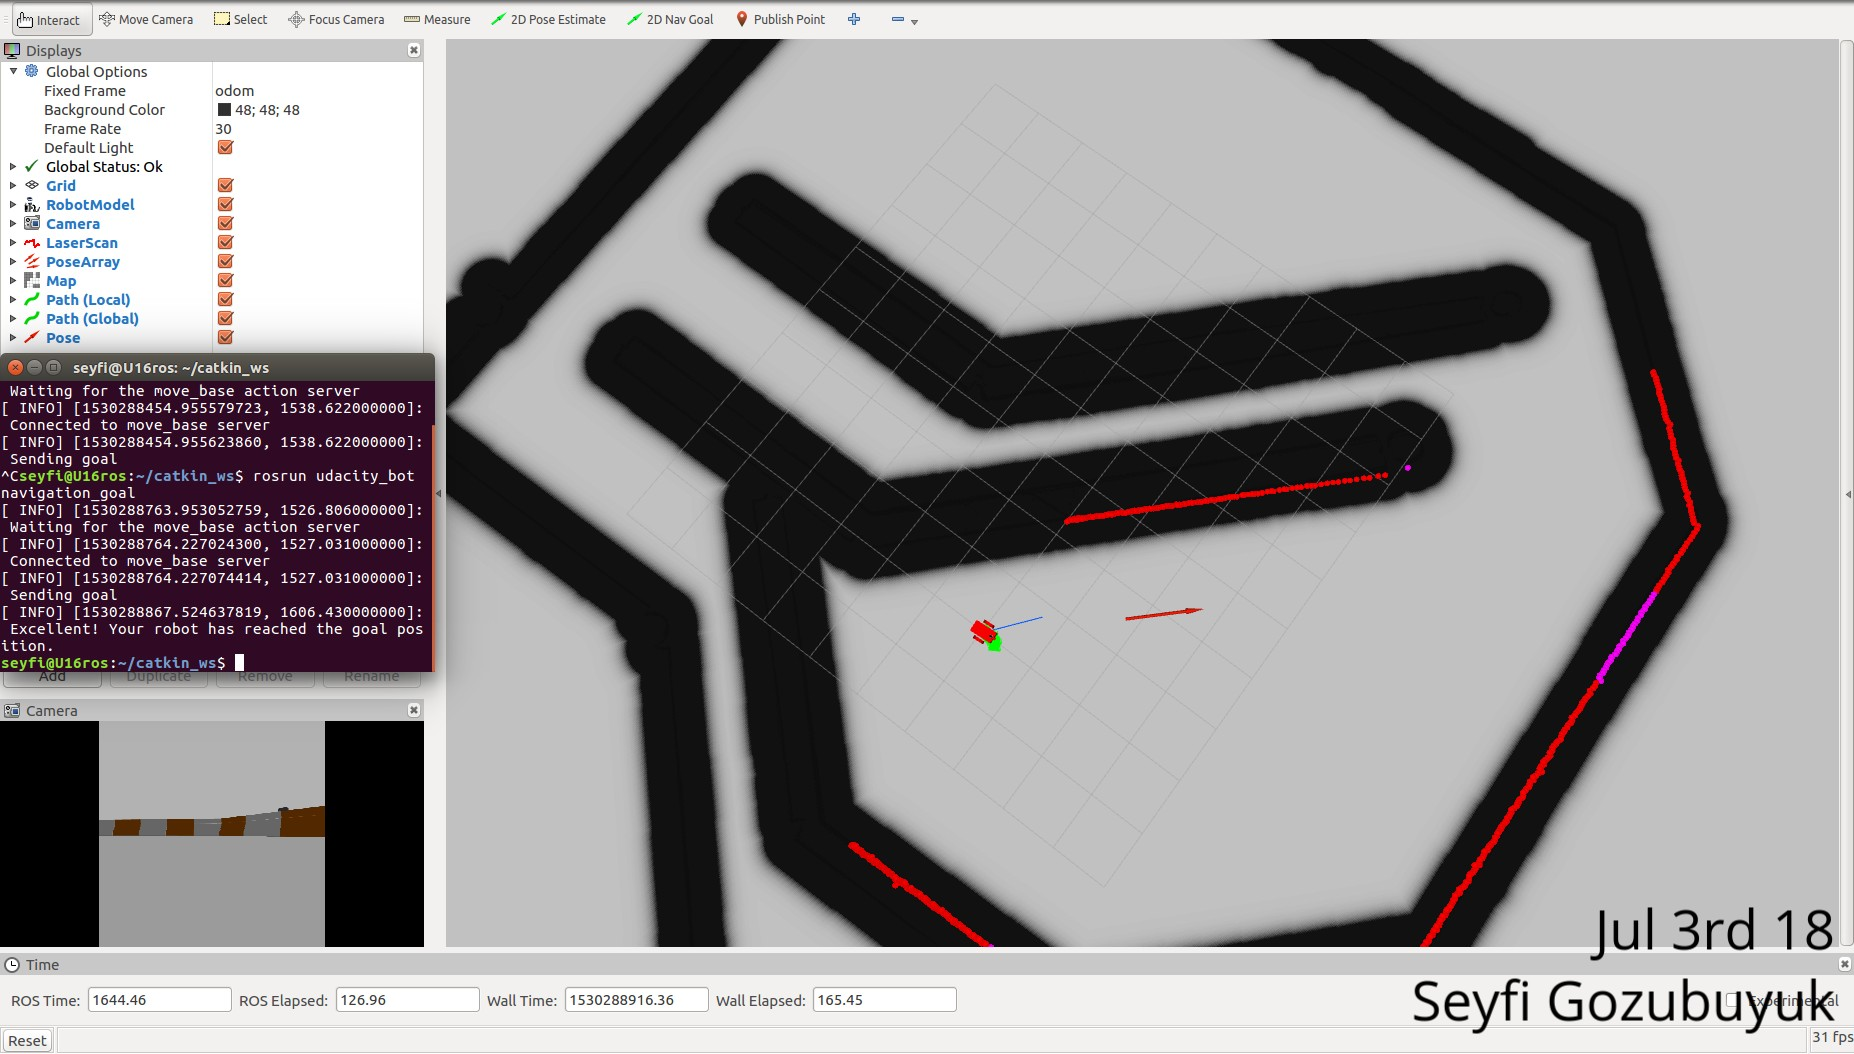
\includegraphics[width=\linewidth]{figures/UdacityBotGoal1.png}
      \caption{Udacity Bot at Goal Run 1}
      \label{fig:ubotgoal1}
\end{figure}


However, on another run it took around 250 seconds, this can be seen from the Figure~\ref{fig:ubotgoal2}. The convergence time for the particles is less then 10 seconds, the Figure~\ref{fig:ubotconv} shows the converged particles. The robot traveled to the opposite direction for 95 seconds. The Figure~\ref{fig:ubotturn} contains the turn back point.

\begin{figure}[thpb]
      \centering
      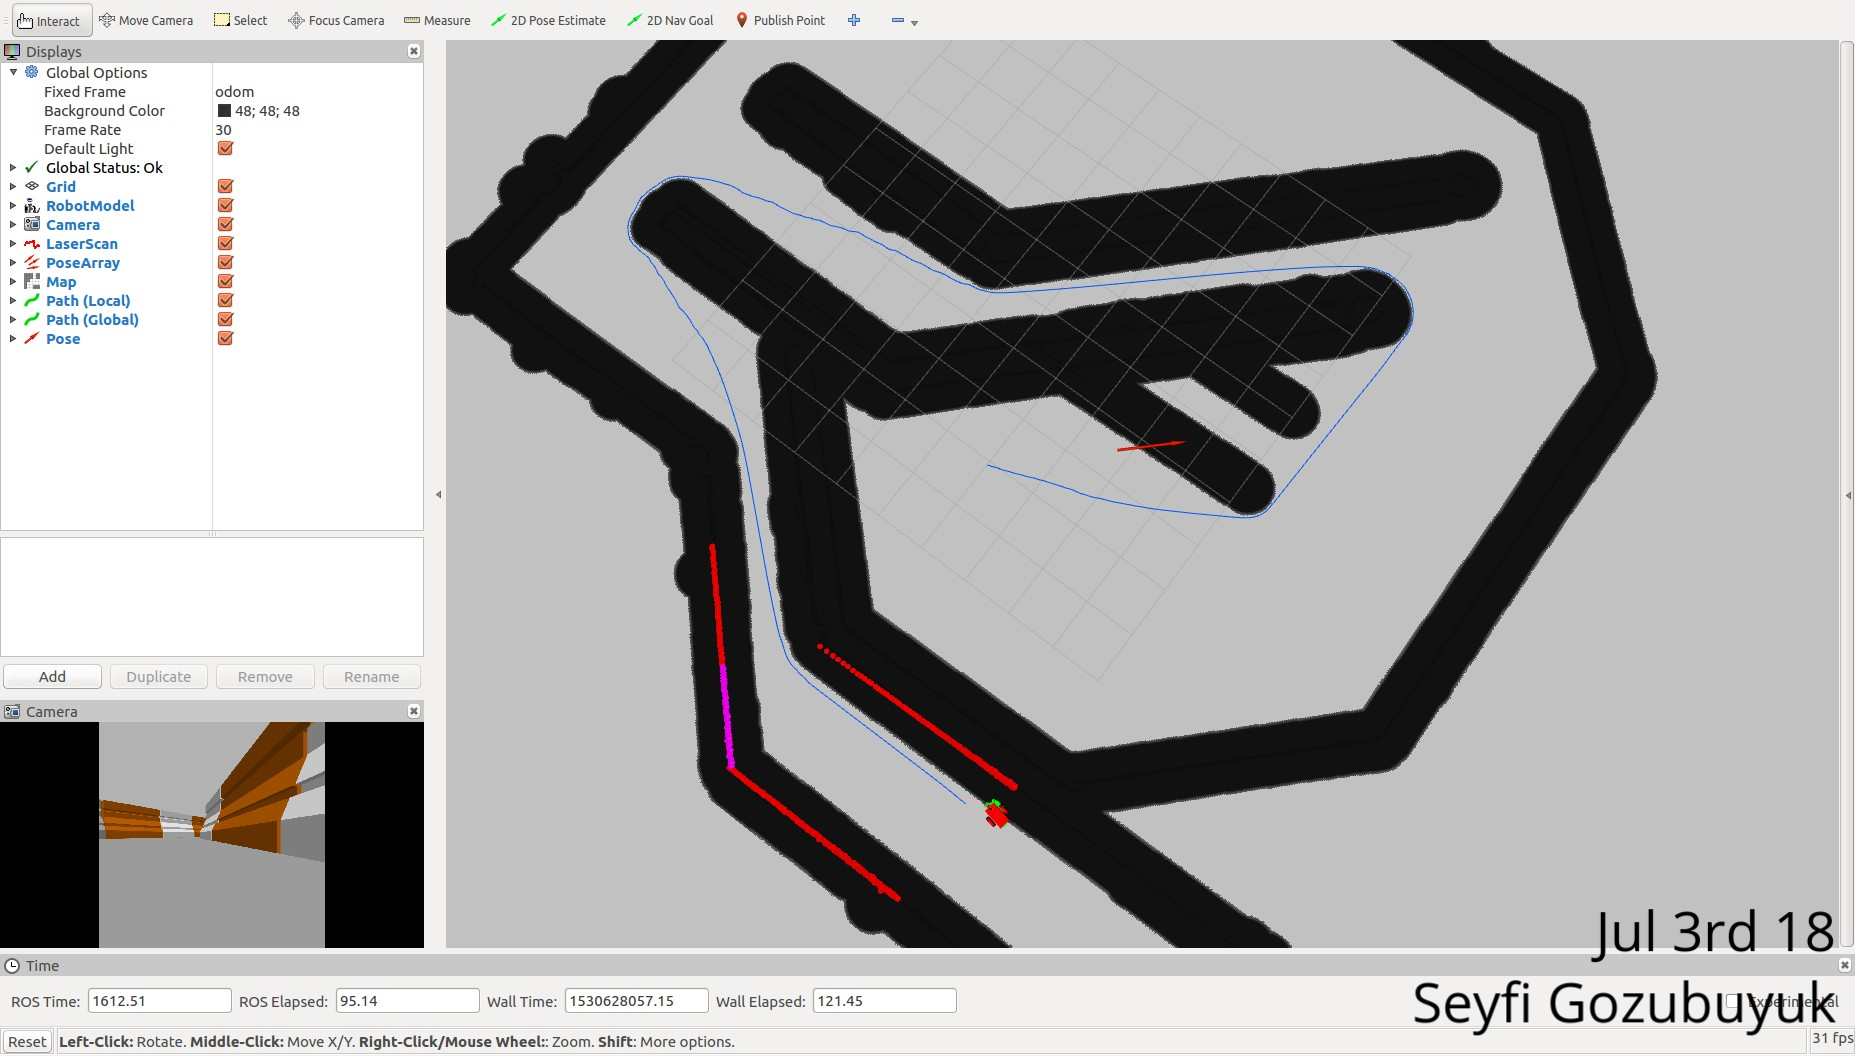
\includegraphics[width=\linewidth]{figures/UdacityBotTurn.png}
      \caption{Udacity Bot - Turn Back}
      \label{fig:ubotturn}
\end{figure}

\begin{figure}[thpb]
      \centering
      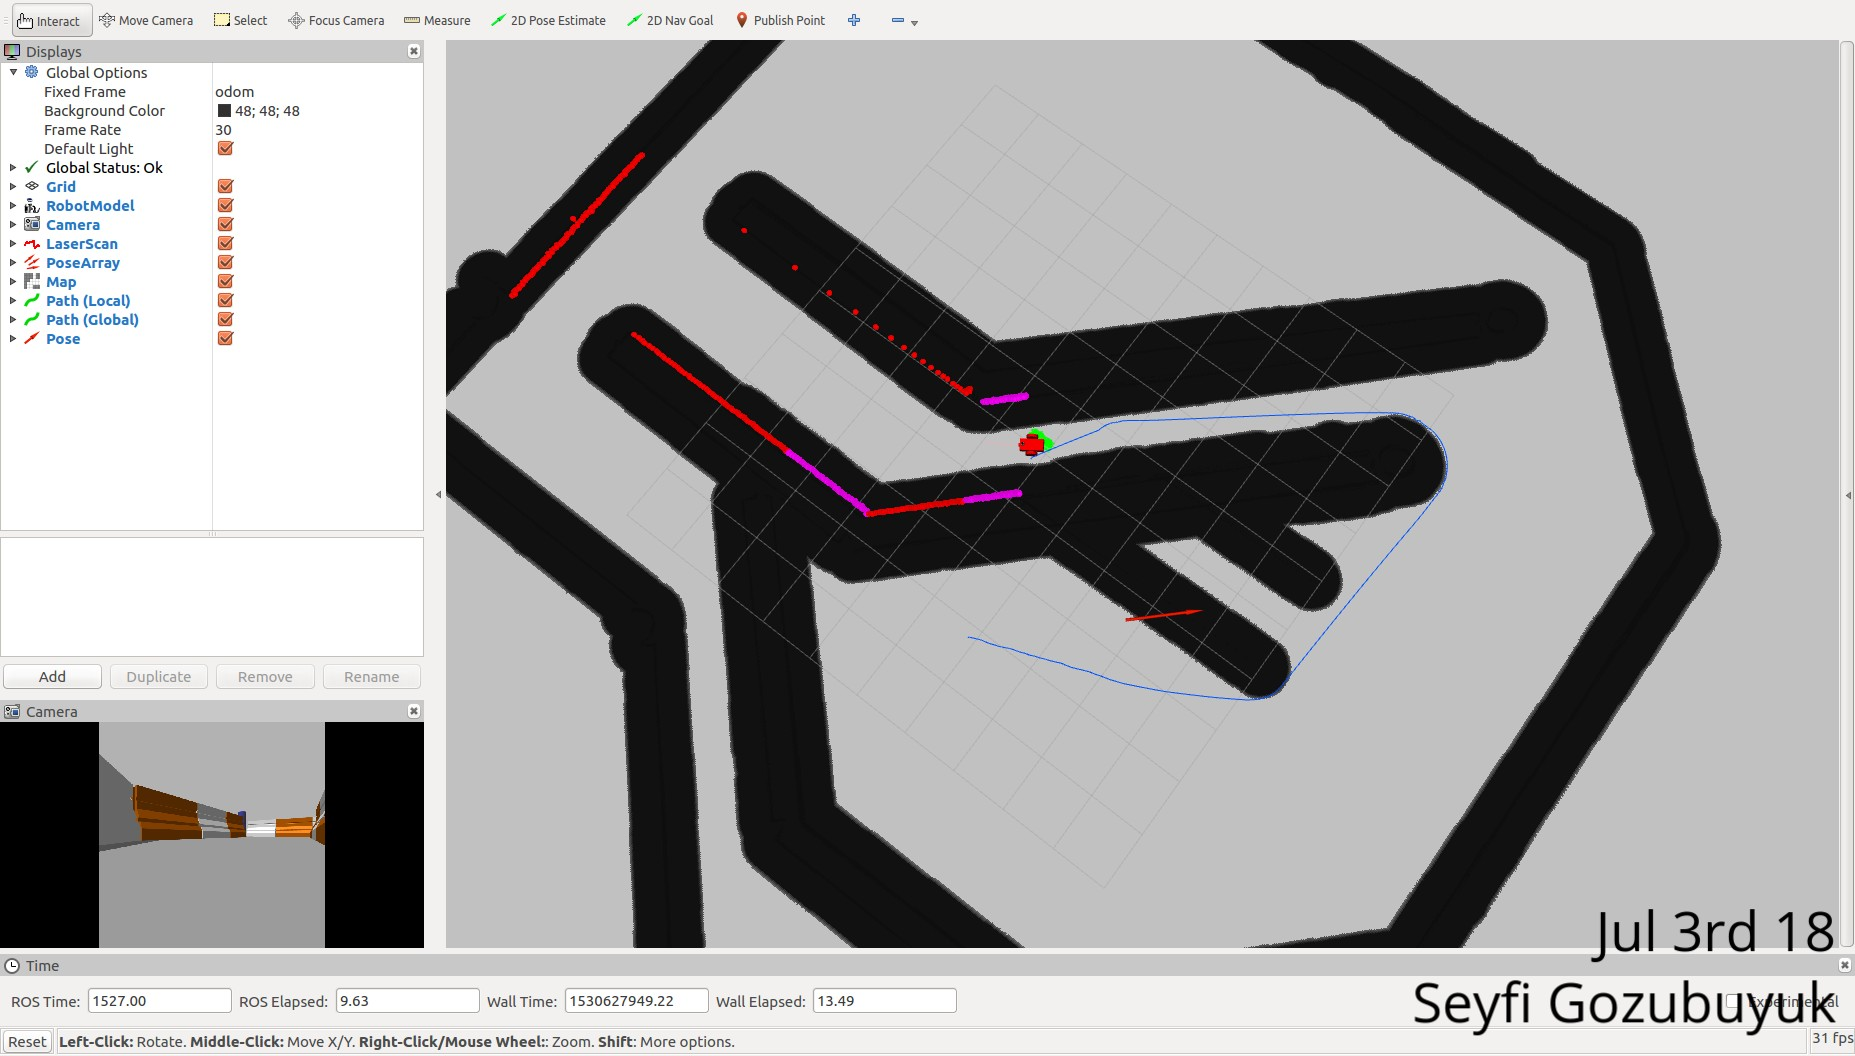
\includegraphics[width=\linewidth]{figures/UdacityBotConv.png}
      \caption{Udacity Bot - Particle Converge}
      \label{fig:ubotconv}
\end{figure}

\begin{figure}[thpb]
      \centering
      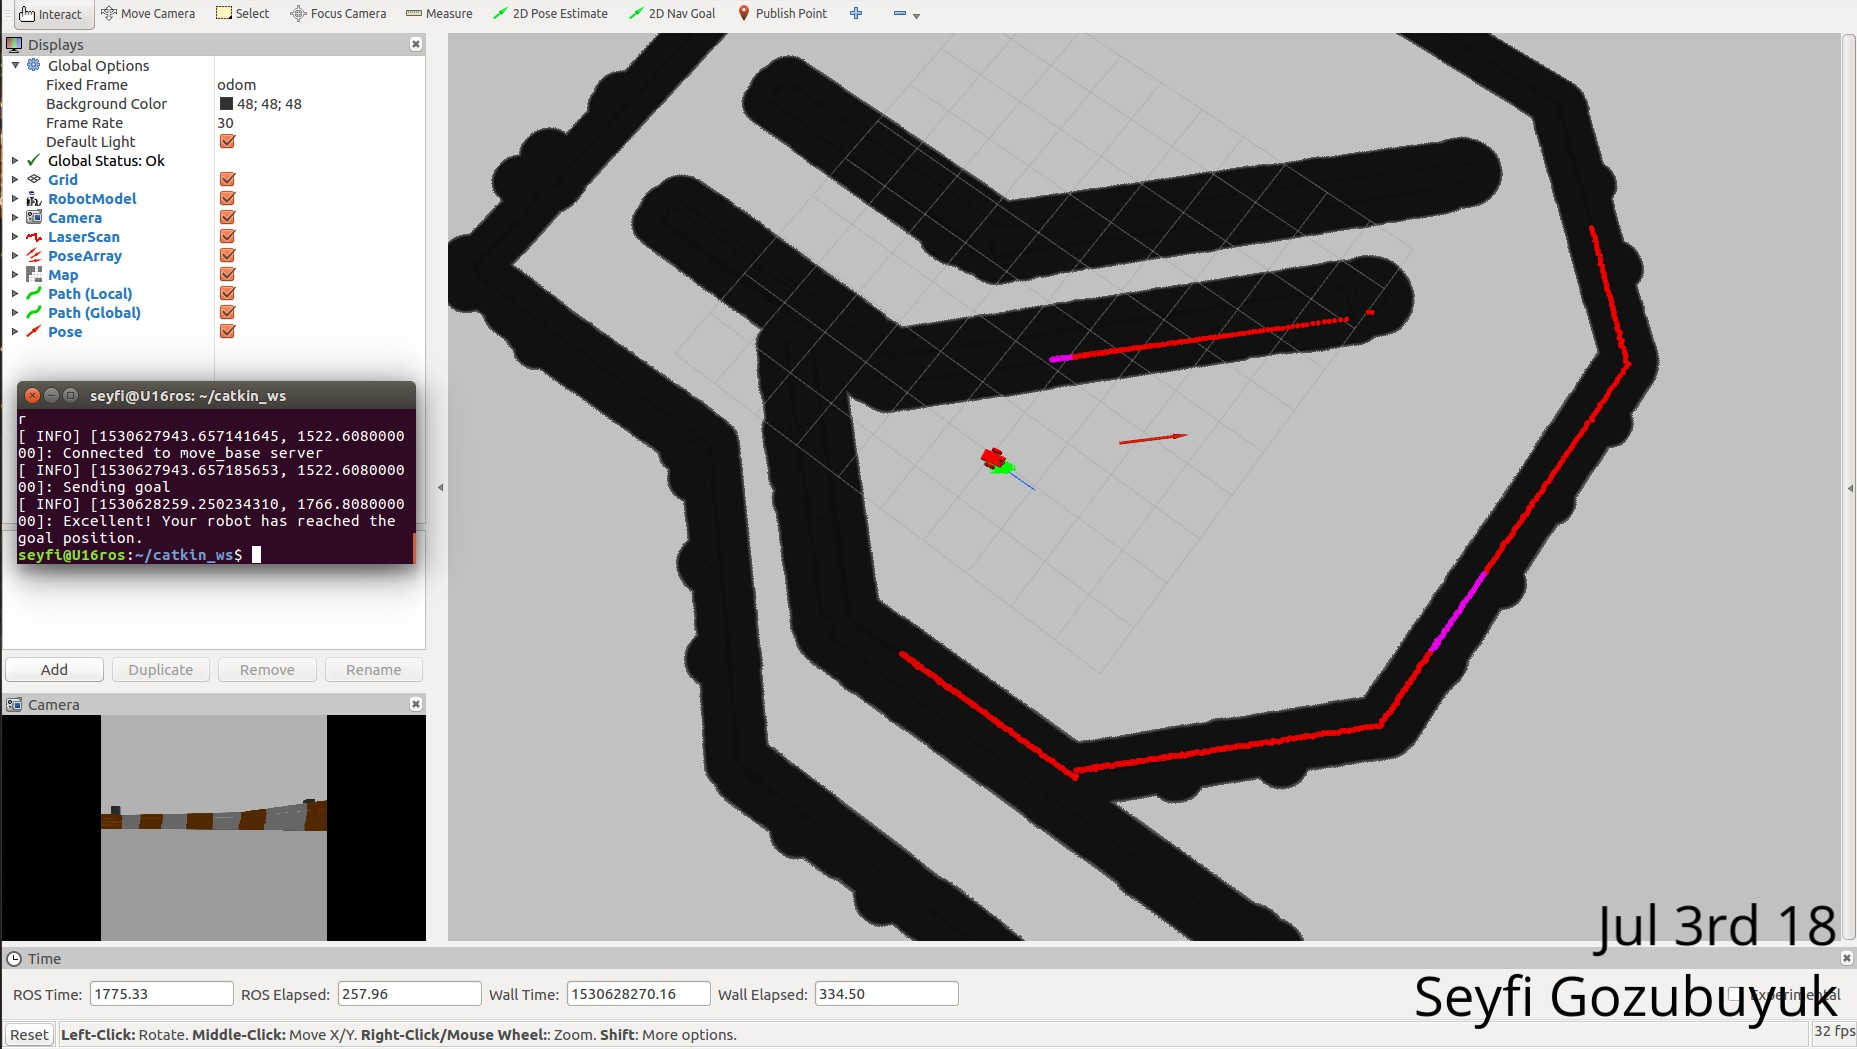
\includegraphics[width=\linewidth]{figures/UdacityBotGoal2.png}
      \caption{Udacity Bot at Goal Run 2}
      \label{fig:ubotgoal2}
\end{figure}

\subsubsection{xbot}
The convergence time of the particles are between 5 seconds and 10 seconds for the xbot, and it is very similar to the one for the Udacity bot. Figure~\ref{fig:xbotconv} shows the particle convergence time for the xbot. xbot reaches to the goal position around 50 to 60 seconds, this can be seen from the Figure~\ref{fig:xbotgoal}.


\begin{figure}[thpb]
      \centering
      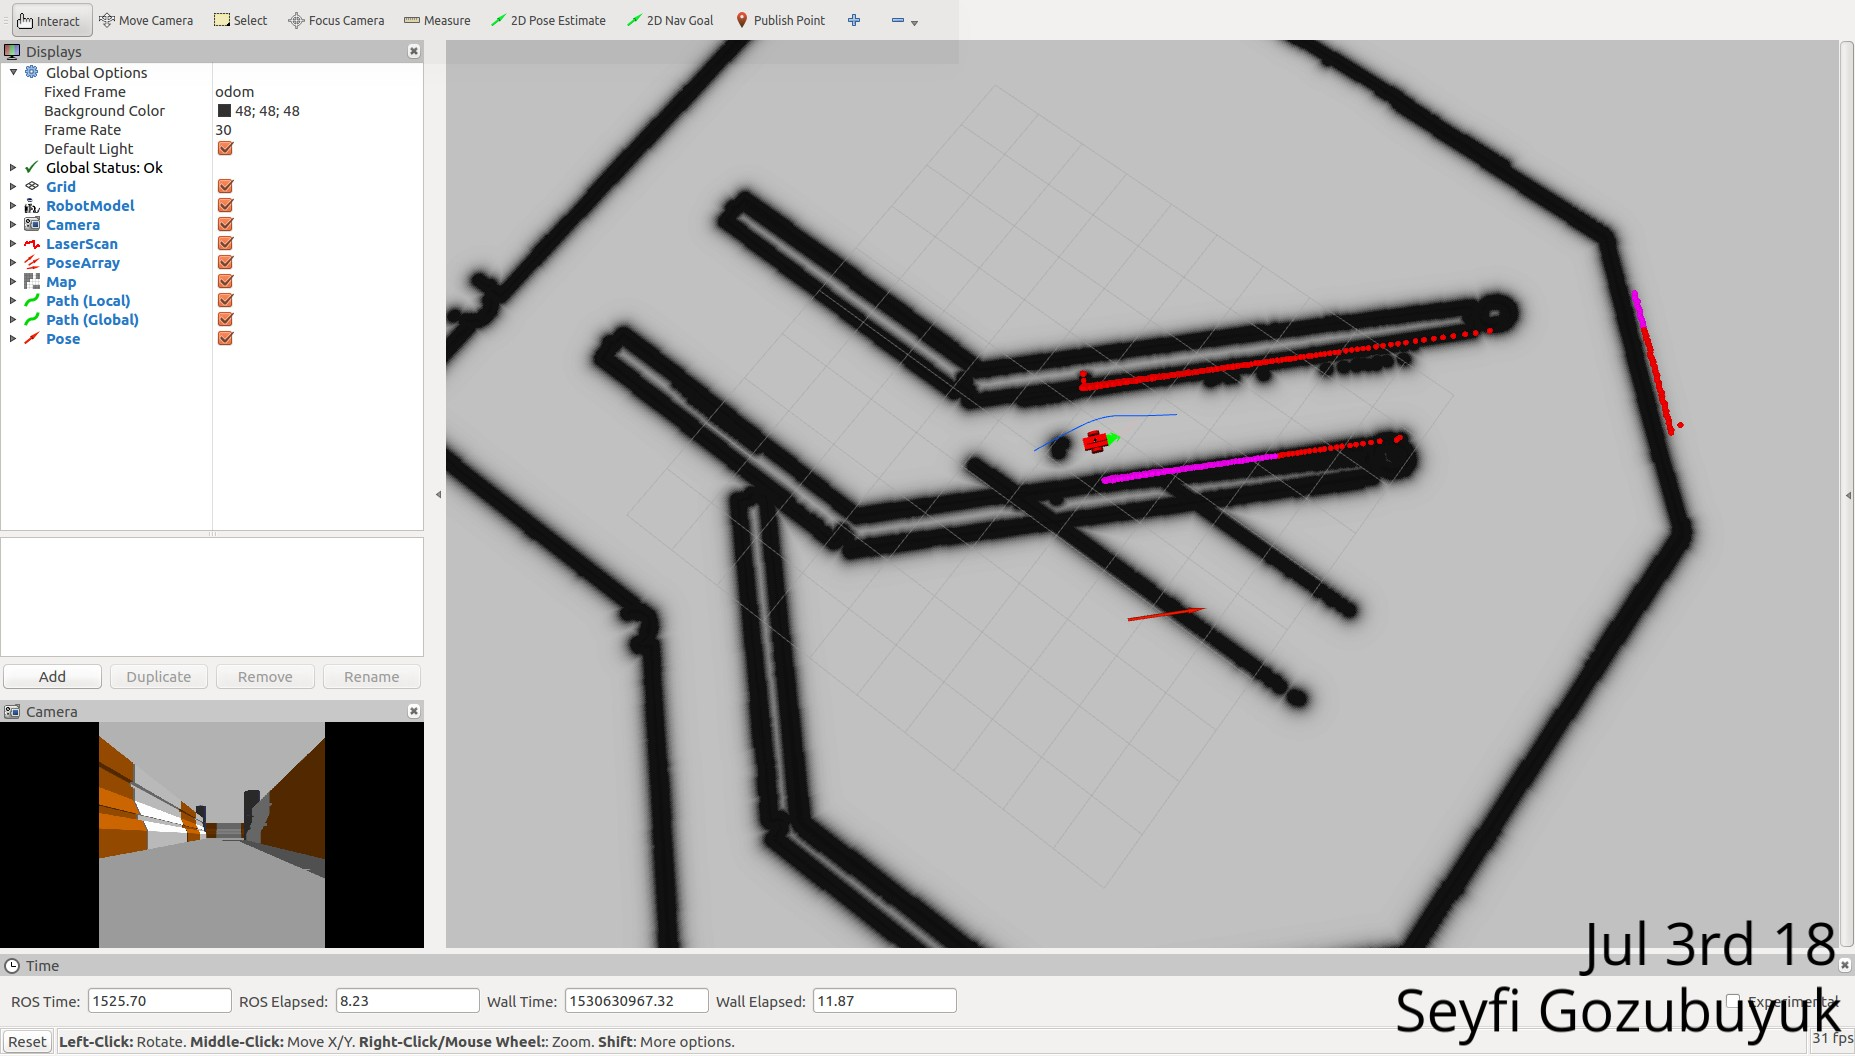
\includegraphics[width=\linewidth]{figures/xbotConv.png}
      \caption{xbot - Particle Converge}
      \label{fig:xbotconv}
\end{figure}

\begin{figure}[thpb]
      \centering
      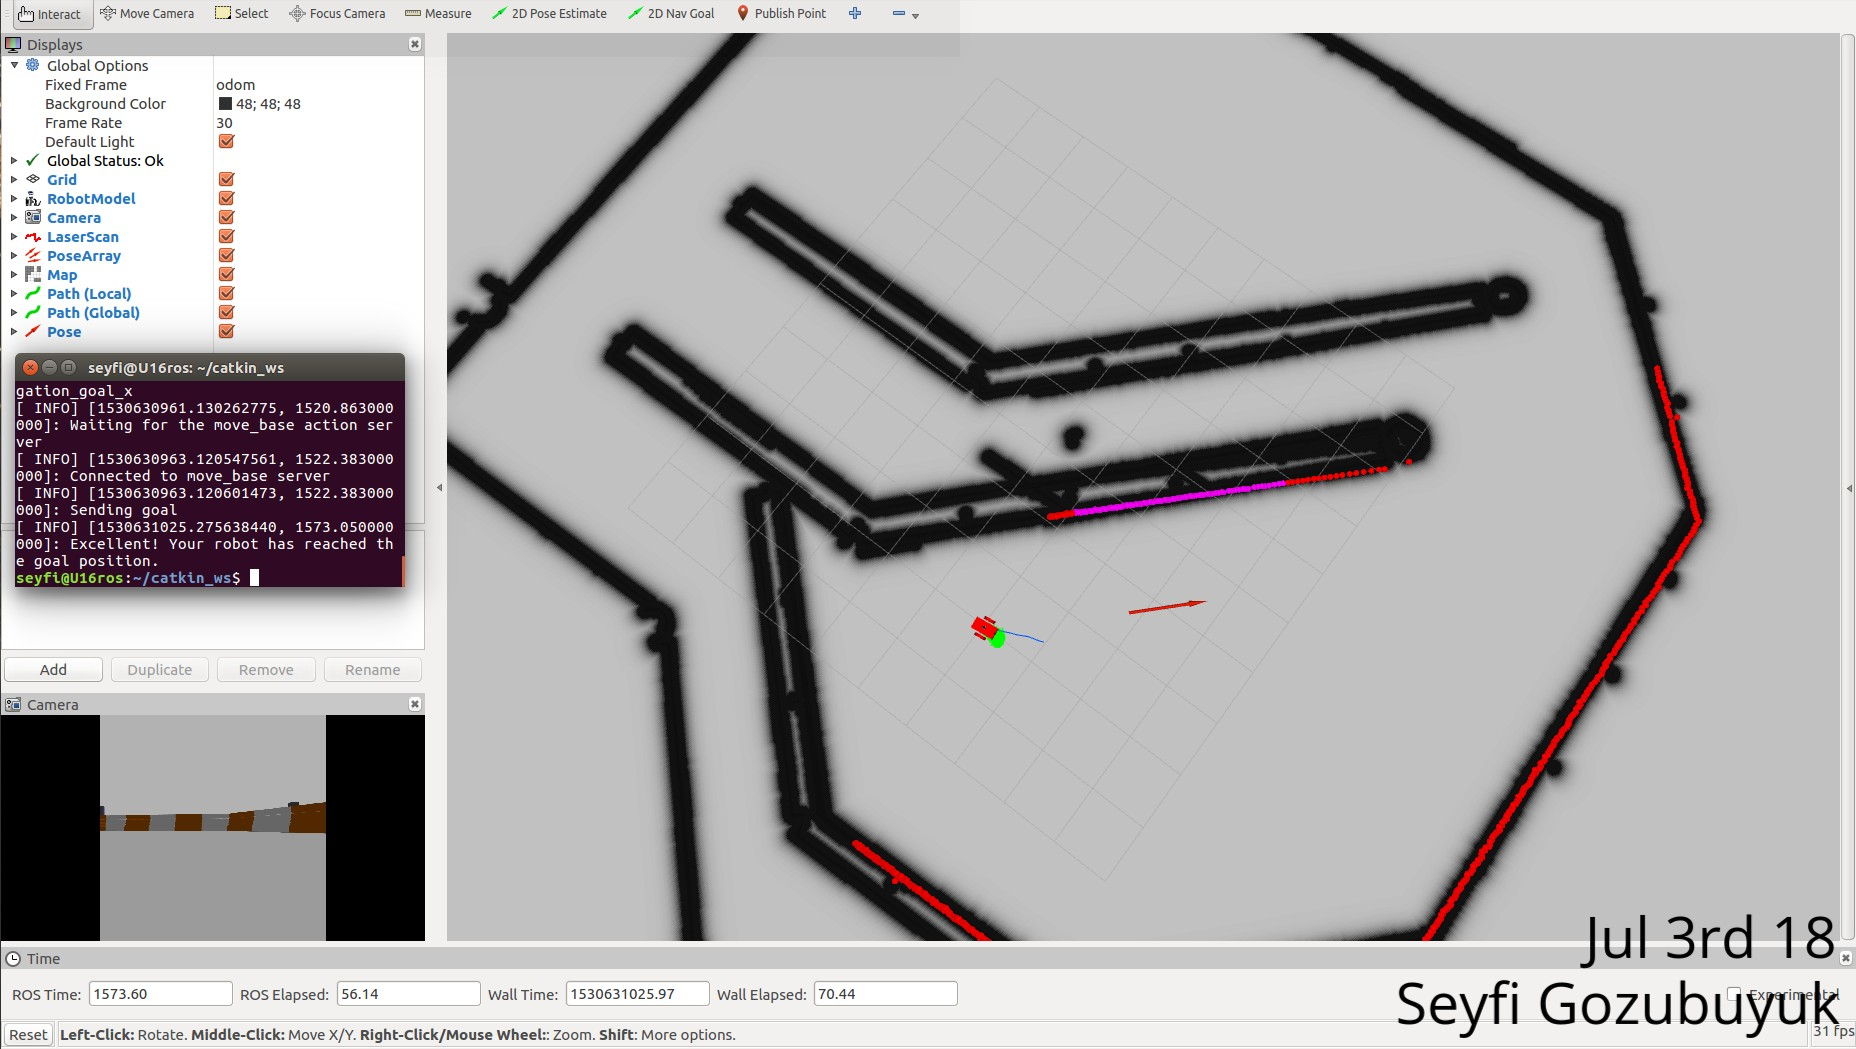
\includegraphics[width=\linewidth]{figures/xbotGoal.png}
      \caption{xbot at Goal}
      \label{fig:xbotgoal}
\end{figure}

\subsection{Technical Comparison} % only facts
The main difference between two robot models is the \textunderscore link, and the sensors are connected to this link, instead of the chassis. There are differences on the parameters selected, which can be seen from the Table~\ref{table:params_ubot_xbot}. The reason for the better performance of the xbot is the differences in the parameters.

\section{Discussion}
The two robot models were able to reach the target. The Udacity Bot first went to opposite direction, whereas the xbot directly moved to the goal direction. The reason for this difference was the differently set parameters. It is required to tune the parameters for the Udacity Bot, but due to time limitations, the tunning operation was marked as a future work. \\
The convergence time for both of the robots were quite similar. Which shows that the AMCL package parameters were almost the same. Actually, only the number of particles parameter was different. As a result, these parameters do not have much effect on localization performance.

\subsection{Topics}
\begin{itemize}
\item xbot performed better. It took less time to reach the goal position.
\item The different costmap parameters let xbot to perform better. The xbot directly started following the global path.
\item The 'Kidnapped Robot' problem is randomly moving the robot to another location. It is a challenge to recover from \cite{wiki:krp}. The current version of the xbot failed to recover from changing its location on Gazebo. The changed position of the xbot is in the Figure~\ref{fig:xbotkidloc}. Figure~\ref{fig:xbotkid1} and Figure~\ref{fig:xbotkid2} show the situation nearly one minute later; and Figure~\ref{fig:xbotkidfail} shows when the AMCL was aborted due to the failure of generating a plan.
\item Localization can be performed in scenarios in which the map is known, and the location of the robot does not randomly change.
\item MCL/AMCL algorithms are a proper choice in industry domains where the map is known and small. The larger the map, the higher the number of particles; which will result in increased computational costs. They work better in closed environments, such as warehouses and stores. The reason for that is to have obstacles, columns, and barriers. The laser sensor will get the distances from them providing more information to localization.
\end {itemize}


\begin{figure}[thpb]
      \centering
      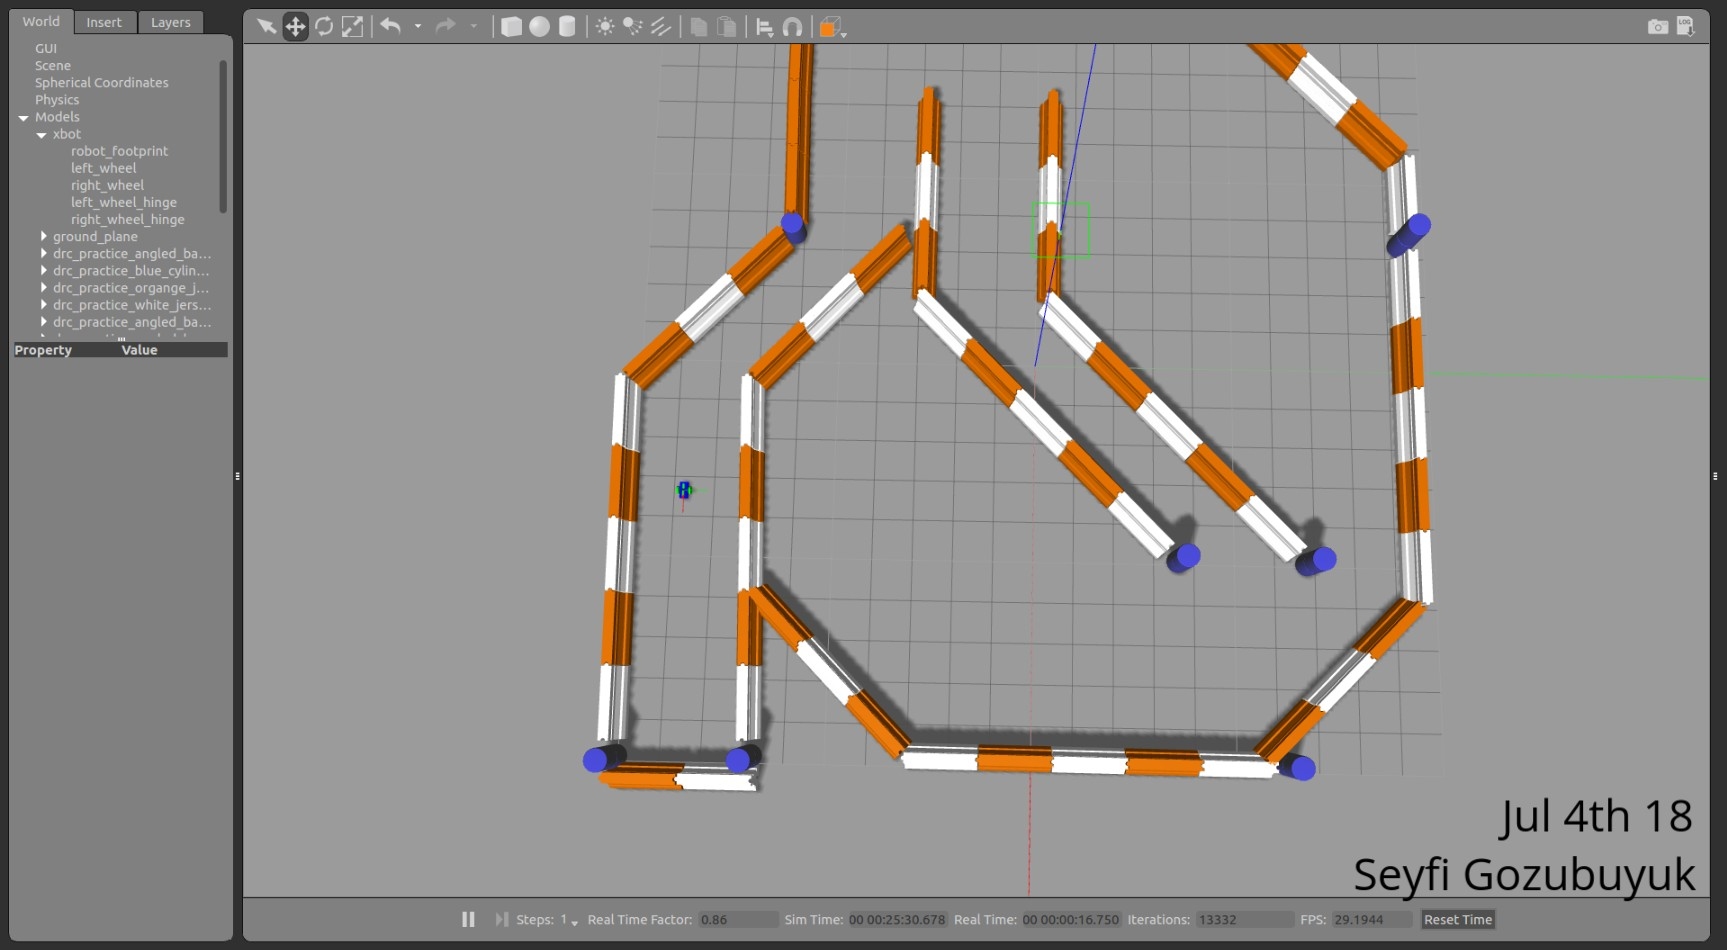
\includegraphics[width=\linewidth]{figures/xbotKidnapLocation.png}
      \caption{xbot - Kidnapped Location}
      \label{fig:xbotloc}
\end{figure}

\begin{figure}[thpb]
      \centering
      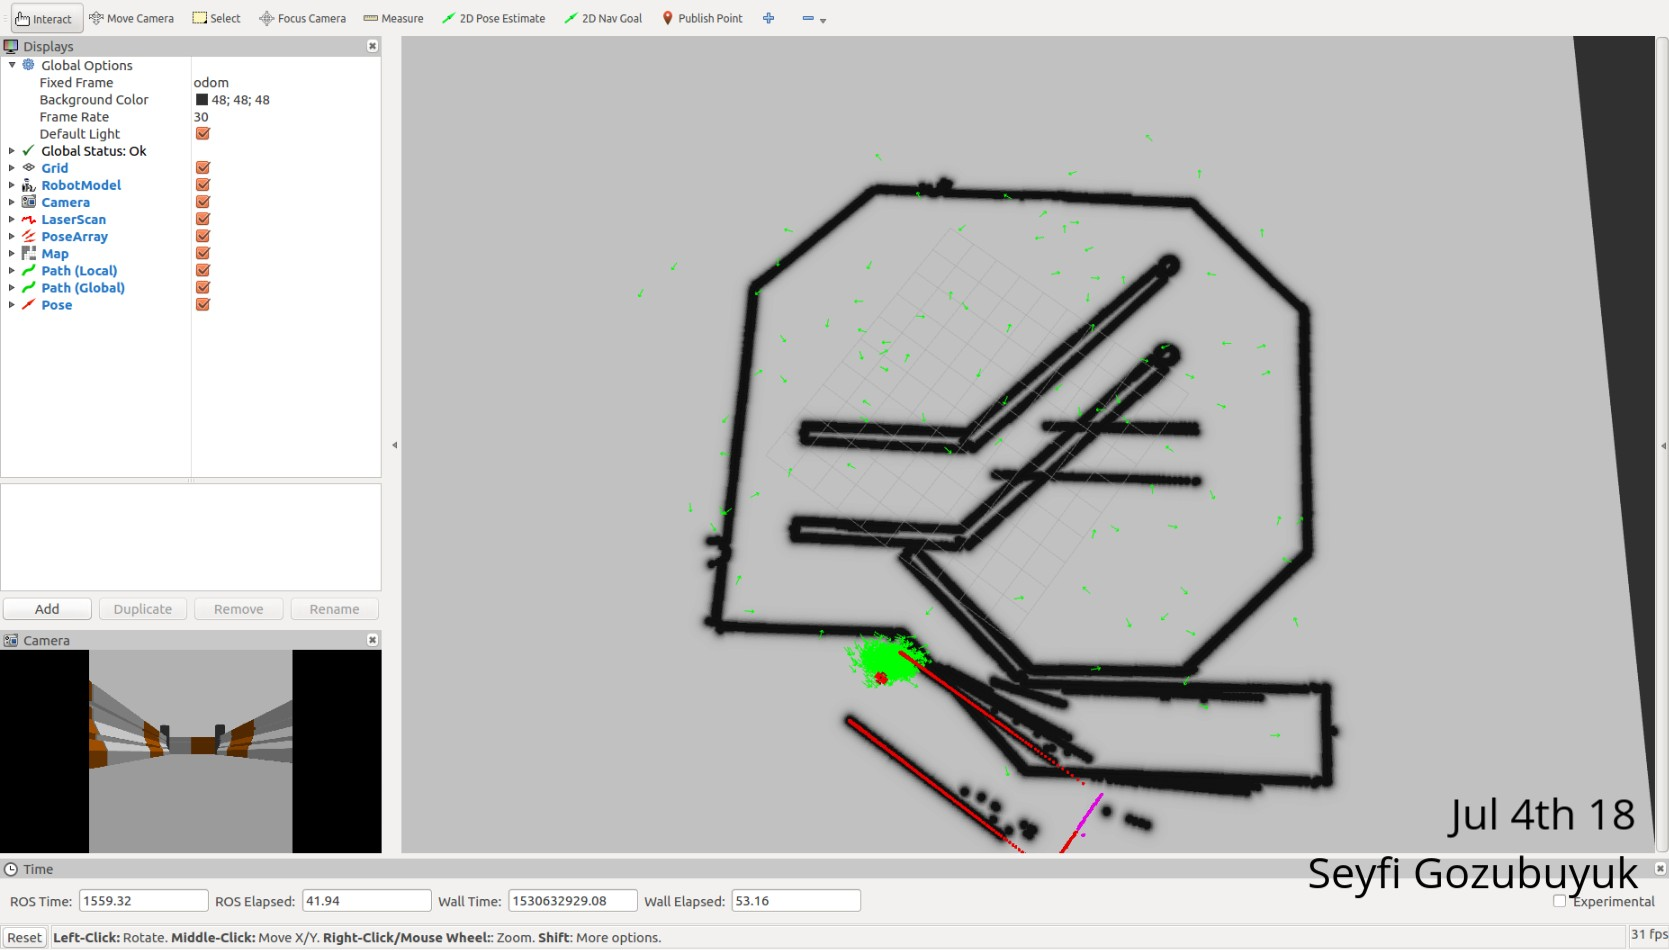
\includegraphics[width=\linewidth]{figures/xbotKidnap1.png}
      \caption{xbot - Kidnapped 1}
      \label{fig:xbotkid1}
\end{figure}

\begin{figure}[thpb]
      \centering
      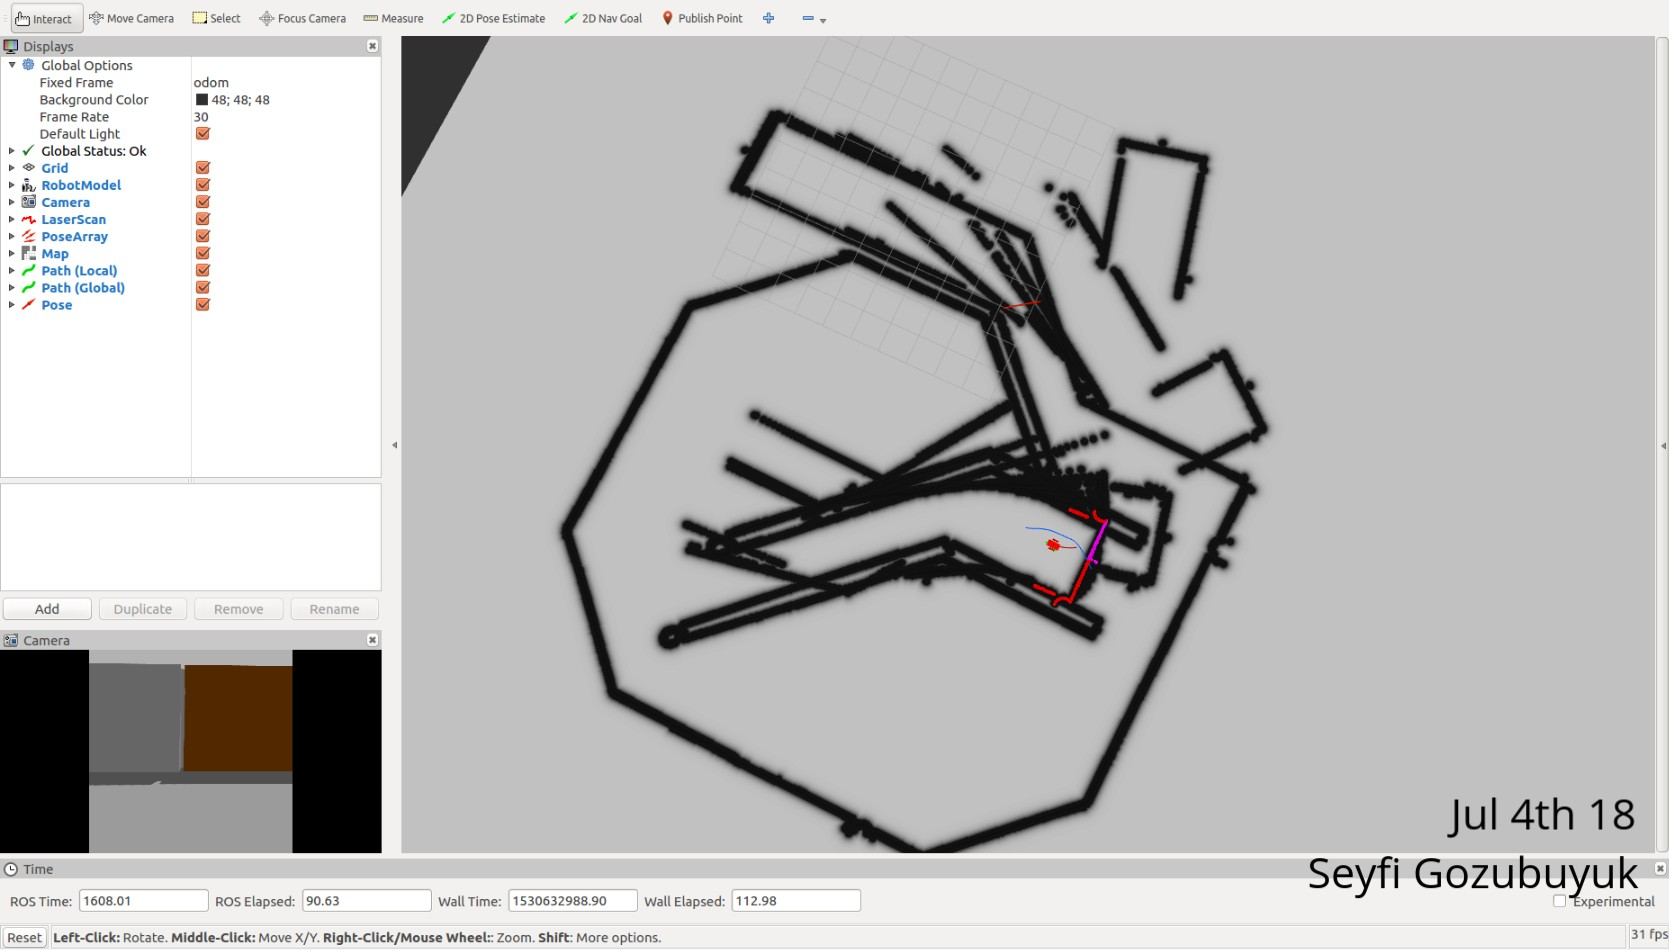
\includegraphics[width=\linewidth]{figures/xbotKidnap2.png}
      \caption{xbot - Kidnapped 2}
      \label{fig:xbotkid2}
\end{figure}

\begin{figure}[thpb]
      \centering
      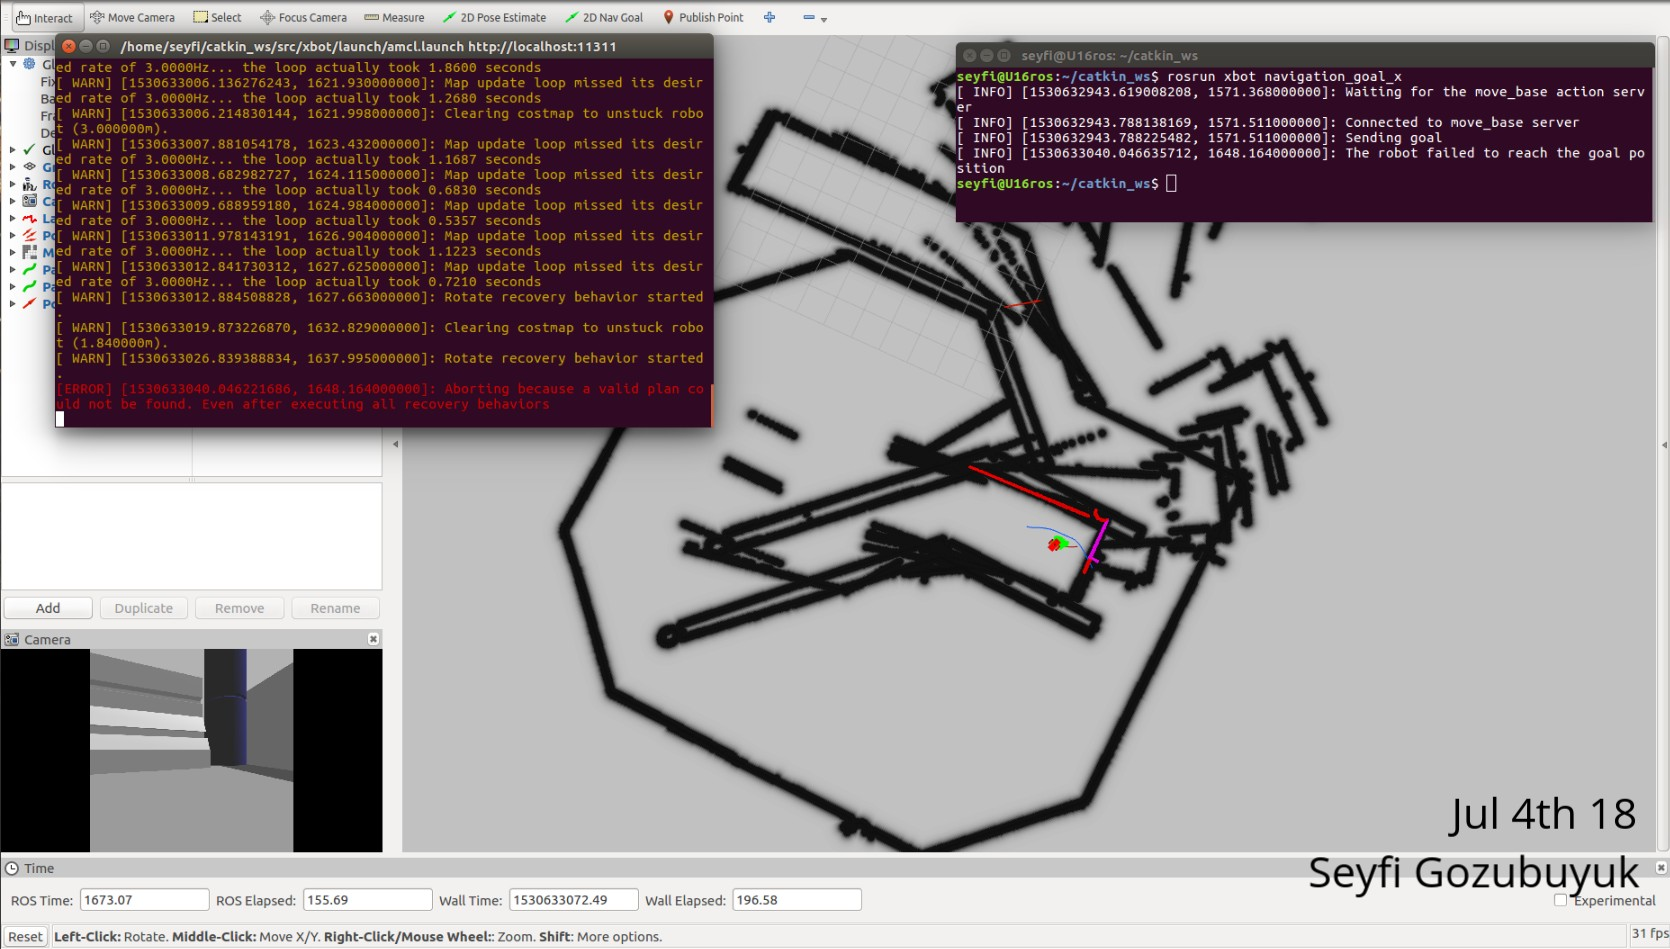
\includegraphics[width=\linewidth]{figures/xbotKidnapFail.png}
      \caption{xbot - Kidnapped Failure}
      \label{fig:xbotkidfail}
\end{figure}

\section{Conclusion / Future work}
It is required to tune the parameters for the Udacity Bot to make it reach the goal position without going the opposite direction first. Another task to work on is kidnapped robot problem. When a robot moved to a random location on Gazebo, it should still be able to reach the target.\\
Testing the algorithm on the Jetson TX2 and comparing the results with the current results is a waiting task for the future work. Upon receiving successful results, the algorithms in the project can be used on a real robot such a vacuum cleaner or an autonomous forklift.


\subsection{Hardware Deployment}
The project was deployed in the simulation environment. The machine has an I7 CPU, 8GB RAM, and 650M GPU. The configuration was able to run the project, but it needed to decrease the update\textunderscore frequency and publish\textunderscore frequency. In addition, there were limitations on the resolution of the costmaps. With more powerful CPU and GPU, it will be possible to increase the update and publish frequencies and the resolutions. Increasing the resolution helped xbot to perform better compared to the Udacity Bot. \\
More powerful hardware will enable to test on different and bigger maps. Using a Jetson TX2 would increase the performance of this project.


\bibliography{bib}
\bibliographystyle{ieeetr}

\end{document}